\documentclass[aspectratio=169]{beamer}
\usepackage[utf8]{inputenc}
\usepackage[english]{babel}
\usepackage{cmap}
\usepackage{eulervm}
\usetheme{Amsterdam_black}
\usepackage{graphicx}
\usepackage{amsmath,amsfonts,amssymb,amsthm,mathtools,pifont,icomma}

\usepackage[natbib=true,backend=biber,bibencoding=utf8,style=authoryear-comp,maxcitenames=2]{biblatex}
\addbibresource{../text/library.bib}

\mathtoolsset{showonlyrefs=true}
\setbeamercovered{transparent}
\setbeamertemplate{navigation symbols}{}

\author{Vladimir Yashin\\ supervised by Geoffrey Decrouez}
\title{Recursive Non-parametric Estimation of the Copula Density}
\institute{Higher School of Economics}
\date{9 June 2018}

\begin{document}
	\maketitle
	
\section{Introduction}
	\subsection{}
		\subsubsection{Marginal and joint PDFs}
			\begin{frame}
				\frametitle{\insertsubsubsection}
				~\\[1em]
				\onslide<1-> What is the joint probability distribution of wage and age? \\[1em]
				
				\onslide<2-> Let us present both random variables in terms of univariate CDFs
				\begin{align}
					F_w(w) &:= \mathbb{P}(W\leq w), \quad \log(w)\sim\mathcal{N}\big(\mu_w, \sigma_w^2\big) \\
					F_a(a) &:= \mathbb{P}(A\leq a), \quad a\sim\mathcal{N}\big(\mu_a, \sigma_a^2\big).
				\end{align}
				
				\onslide<3-> Then, the joint distribution has the following form
				\begin{align}
					F(w, a) := \mathbb{P}(W\leq w, A\leq a).
				\end{align}

			\end{frame}
		
		\subsubsection{Marginal and joint PDFs of independent samples}
			\begin{frame}
				\frametitle{\insertsubsubsection}				
				
				\onslide<1-> 
				\begin{center}
					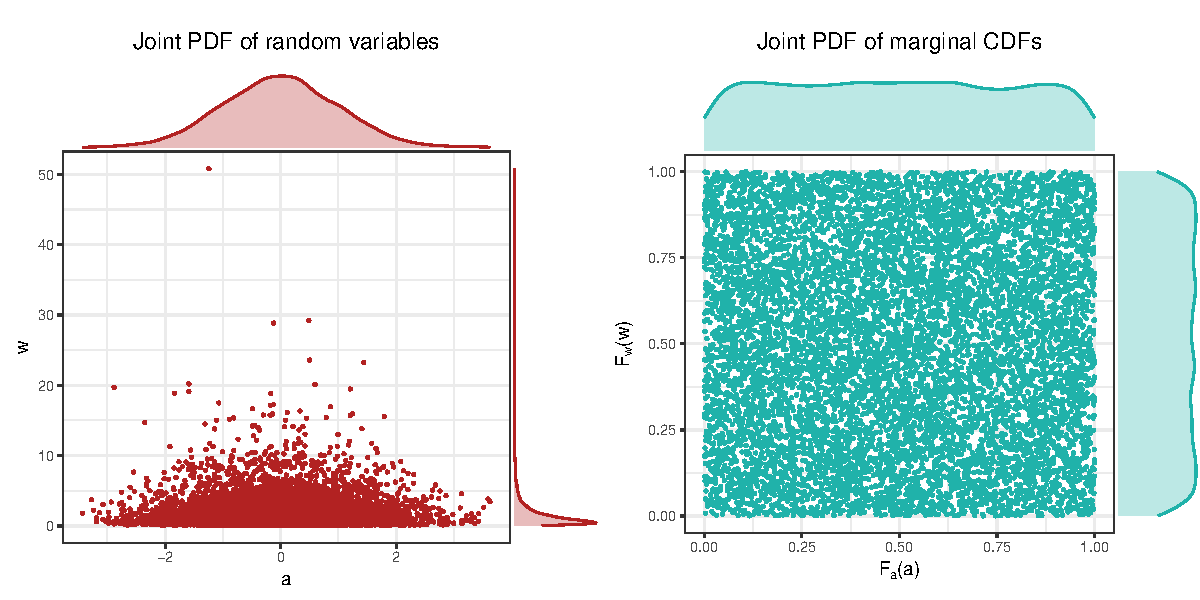
\includegraphics[width=0.95\linewidth]{plots/introduction/indep}
				\end{center}
				
			\end{frame}
			
		\subsubsection{Marginal and joint PDFs of dependent samples ($ \rho = 0.8 $)}
			\begin{frame}
				\frametitle{\insertsubsubsection}				
				
				\onslide<1-> 
				\begin{center}
					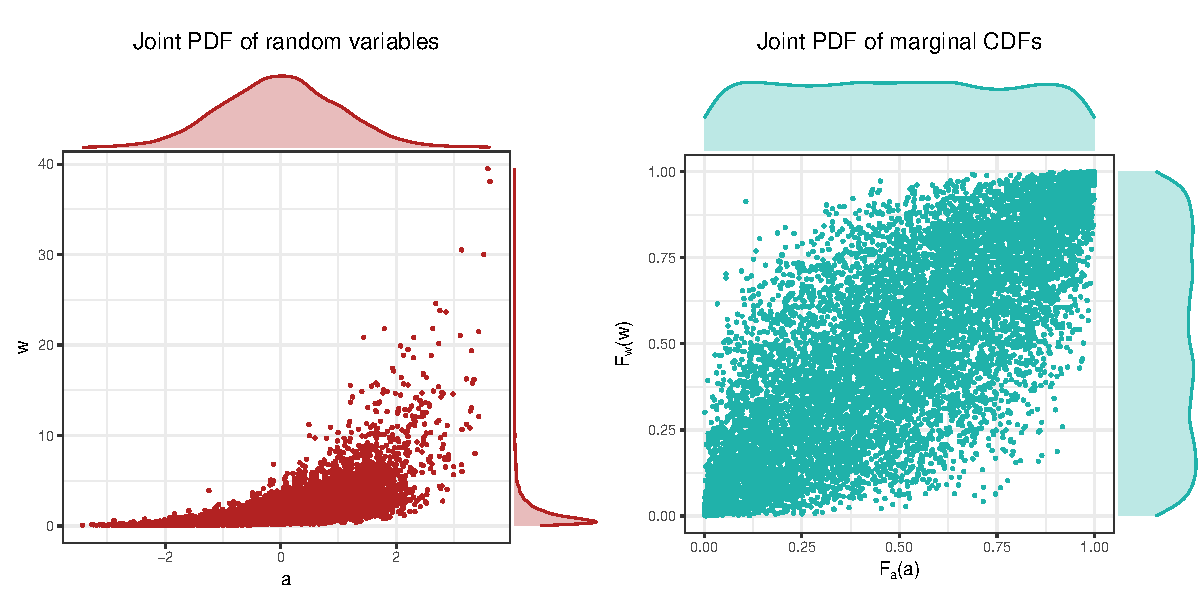
\includegraphics[width=0.95\linewidth]{plots/introduction/dep}
				\end{center}
				
			\end{frame}
	
		\subsubsection{How to measure dependence between variables?}
			\begin{frame}
				\frametitle{\insertsubsubsection}
				
				\onslide<1-> We wish to describe dependence structure between $ w $ and $ a $. What to do? \\[1em]
				
				\onslide<2-> $ 1^\text{st} $ idea: Pearson correlation coefficient (\ding{55}: non-linear dependence); \\[1em]
				
				\onslide<3-> $ 2^\text{nd} $ idea: Spearman's rank correlation coefficient (\ding{55}: information is too general); \\[1em]
				
				\onslide<4-> $ 3^\text{rd} $ idea: to consider joint PDF of marginals (\ding{55}: family of CDFs are rarely known).
				
			\end{frame}
			
		\subsubsection{Let's use copulas}
			\begin{frame}
				\frametitle{\insertsubsubsection}
				
				\onslide<2->{Copulas can address these problems}
				\begin{itemize}
					\item[]<3-> \ding{51}: can capture non-linear dependence;
					\item[]<4-> \ding{51}: shows rich visual information of dependence structure;
					\item[]<5-> \ding{51}: marginals might be of non-parametric families.
					
				\end{itemize}
				
			\end{frame}
			
		\subsubsection{What are copulas?}
			\begin{frame}
				\frametitle{\insertsubsubsection}
				~\\[1em]
				Copula is a multivariate CDF such that a marginal CDF for each variable is uniform. \\[1em]
				
				\begin{center}
					
\includegraphics[width=0.75\linewidth]{plots/introduction/blank}
				\end{center}
				
			\end{frame}
			
			\begin{frame}
				\frametitle{\insertsubsubsection}
				~\\[1em]
				Copula is a multivariate CDF such that a marginal CDF for each variable is uniform. \\[1em]
				
				\begin{center}
					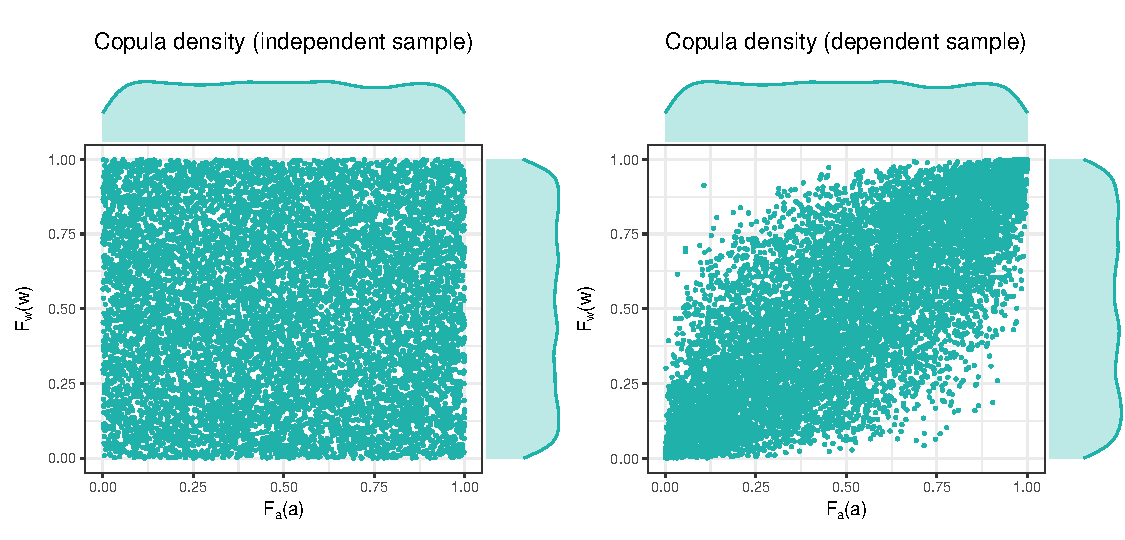
\includegraphics[width=0.75\linewidth]{plots/introduction/copulas}
				\end{center}
				
			\end{frame}
			
		\subsubsection{Let's get technical}
			\begin{frame}
				\frametitle{\insertsubsubsection}
				
				\onslide<2-> There exists\footcite{Sklar1959} a unique $ d $-variate copula $ C: [0, 1]^d \rightarrow [0, 1] $ such that
				\begin{align}
					F(X_1, \dots, X_d) = C\big(F_1(X_1), \dots, F_d(X_d)\big),
				\end{align}
				where $ (X_1, \dots, X_d) $ is a set of $ d $ random variables like age, wage, etc.\\[1em]
				
				\onslide<3-> Therefore, the copula density 
				\begin{align}
					c\big(F_1(X_1), \dots, F_d(X_d)\big) = \frac{f(X_1, \dots, X_d)}{\prod_{j=d}^{d}f_j(X_j)}
				\end{align}
				
			\end{frame}
			
		\subsubsection{Why old methods are bad?}
			\begin{frame}
				\frametitle{\insertsubsubsection}
				
				The existing copula estimators are not on-line. \\[1em]
				
				Therefore, it has to be entirely recalculated in case of persistent data flow.
				
			\end{frame}
	
\section{Copula Density Estimator}
	\subsection{}
		\subsubsection{How to estimate copula density?}
			\begin{frame}
				\frametitle{\insertsubsubsection}
				
				Recall that
				\begin{align}
					c\big(F_1(X_1), \dots, F_d(X_d)\big) = \frac{f(X_1, \dots, X_d)}{\prod_{j=d}^{d}f_j(X_j)}.
				\end{align}
				\\[1em]
				First, we need to recursively estimate joint PDF $ f $ and each of marginal PDFs $ f_j $.
				
			\end{frame}
				
		\subsubsection{Robbins-Monro procedure}
			\begin{frame}
				\frametitle{\insertsubsubsection}
				
				\onslide<1-> A root of unknown function $ h $ using only noisy observations can be found as follows\footcite{Robbins1951}
				\begin{align}
					z_n = z_{n-1} - \alpha_n H(z_n, \varepsilon_n)
				\end{align}
				where $ H(z_n, \varepsilon_n) \equiv (h(z_n) + \varepsilon_n) $ is a noisy observation and $ \alpha_n $ is a sequence of positive numbers that converges to 0. \\[1em]
				
				\onslide<2-> It was proved that $ z_n $ converges almost surely to $ z^\star $ as $ n\rightarrow \infty $, given $ \mathbb{E}[\varepsilon]=0 $.
				
			\end{frame}
		
		\subsubsection{Quantile estimation using Robbins-Monro procedure}
			\begin{frame}
				\frametitle{\insertsubsubsection}
				
				To estimate a PDF we first need to estimate quantiles.
				\\[1em]
				
				
				\onslide<2-> An estimator of $ u $-th quantile can be derived from the Robbins-Monro procedure
				\begin{align}
					x^u_n = x^u_{n-1} + \alpha_n\big(u - \mathbf{1}(X_{n-1}\leq x^u_{n-1})\big),
				\end{align}
				where $ x^u_n $ is a $ u $-th quantile estimator.
				
			\end{frame}
			
			
		\subsubsection{Smoothed recursive non-parametric estimation of marginal PDFs $ f_j $}
			\begin{frame}
				\frametitle{\insertsubsubsection}
				
				A smoothed adaptation of the quantile estimator\footnote{Definition and a proof of convergence in \textcite{Amiri2014}}
				\begin{align}
					f^{u_j}_{j, n} &= (1- 1/n) \cdot f^{u_j}_{j, n-1} + 1/n \cdot K^{u_j}_{h_{j, n}}\big(x^{u_j}_{n-1} - X_{n, j}\big) \\
					a^{u_j}_{j, n} &= \max\Big[\mu_{j, n}, \min\big[f^{u_j}_{j, n}, \nu \ln(n+1)\big]\Big] \\
					x^{u_j}_n &= x^{u_j}_{n-1} + \frac{1}{n a^{u_j}_{j, n}}\Big[u_j - \mathbf{1}\big(X_{n, j}\leq x^{u_j}_{n-1}\big)\Big],
				\end{align}
				where $ K_{h_{j, n}}^{u_j}(\cdot) $ is a symmetric, univariate kernel with bandwidth $ h_{j,n} $;\\ $ \mu_{j, n} $ and $ \nu $ are some positive constants.
				
			\end{frame}			
			
		\subsubsection{Smoothed recursive non-parametric estimation of joint PDF $ f $}
			\begin{frame}
				\frametitle{\insertsubsubsection}
				
				A recursive estimator for the joint PDF defined as follows\footnote{Definition and a proof of convergence in \textcite{Mokkadem2009}}
				\begin{align}
					f^{\mathbf{u}}_n &= (1- 1/n) \cdot f^{\mathbf{u}}_{n-1} + 1/n \cdot \mathbf{K}_{b_n}^{\mathbf{u}} \big(x_{n-1}^{\mathbf{u}} - \mathbf{X}_n\big),
				\end{align}
				where now instead of $ u_j $ we have a grid of points $ \mathbf{u} $ and multivariate data point $ \mathbf{X}_n $; \\
				$ \mathbf{K}_{b_n}^{\mathbf{u}}(\mathbf{X}) := \prod_{j=1}^{d}K_{b_{n}}^{u_j}(\mathbf{X}_j) $ where $ K_{b_{n}}^{u_j}(\mathbf{X}_j) $ is a univariate kernel with bandwidth $ b_{n} $.
				
			\end{frame}
			
			
		\subsubsection{Some remarks on marginal and joint PDFs estimators}
			\begin{frame}
				\frametitle{\insertsubsubsection}
				
				\begin{align}
					f^{u_j}_{j, n} &= (1- 1/n) \cdot f^{u_j}_{j, n-1} + 1/n \cdot K^{u_j}_{h_{j, n}}\big(x^{u_j}_{n-1} - X_{n, j}\big) \\
					f^{\mathbf{u}}_n &= (1- 1/n) \cdot f^{\mathbf{u}}_{n-1} + 1/n \cdot \mathbf{K}_{b_n}^{\mathbf{u}} \big(x_{n-1}^{\mathbf{u}} - \mathbf{X}_n\big),
				\end{align}\\[1em]
				
				Remarks:
				\begin{itemize}
					\item<2-> The marginal estimator is just a special case of the joint estimator;
					\item<3-> The authors of the joint estimator didn't provide the estimation for quantiles $ x^{\mathbf{u}} $;
					\item<4-> Therefore, the estimation of the quantile $ x^{u_j} $ has to be generalized \ding{51}.
				\end{itemize}
				
			\end{frame}
			
		\subsubsection{Recursive non-parametric copula density estimator}
			\begin{frame}
				\frametitle{\insertsubsubsection}
				~\\
				Given
				\begin{align}
					f^{u_j}_{j, n} &= (1- 1/n) \cdot f^{u_j}_{j, n-1} + 1/n \cdot K^{u_j}_{h_{j, n}}\big(x^{u_j}_{n-1} - X_{n, j}\big), \\
					f^{\mathbf{u}}_n &= (1- 1/n) \cdot f^{\mathbf{u}}_{n-1} + 1/n \cdot \mathbf{K}_{b_n}^{\mathbf{u}} \big(x_{n-1}^{\mathbf{u}} - \mathbf{X}_n\big),
				\end{align}
				$ c_n(\cdot) $ defined as follows
				\begin{align}
					c_n &= \frac{f^{\mathbf{u}}_n}{\prod_{j=1}^{d}f^{u_j}_{j, n}}
				\end{align}
				to the best of our knowdlenge, is the first recursive non-parametric estimator of the copula density $ c(\cdot) $\\[-4ex]
				\begin{align}
					c = \frac{f}{\prod_{j=d}^{d}f_j}.
				\end{align}
				
			\end{frame}
			
		
\section{Bandwidth Selection}
	\subsection{}
		\subsubsection{How to select the bandwidths?}
			\begin{frame}
				\frametitle{\insertsubsubsection}
				
				We have two sets of bandwidths $ h_j $ for each of marginals and $ b $ for the joint. \\[1em]
				
				\onslide<2-> Two groups of bandwidths:
				\begin{itemize}
					\item Data-independent;
					\item Data-dependent.
				\end{itemize}
				
			\end{frame}
			
		\subsubsection{Constant bandwidth}
			\begin{frame}
				\frametitle{\insertsubsubsection}
				
				The simplest data-independent case: $ h_j $ and $ b $ are the same\footnote{As proposed in \textcite{Robinson1975} and \textcite{Holst1987} for non-smooth recursive algorithms.} and calculated as follows
				\begin{align}
					b_n = h_{j,n} = n^{-\tau},
				\end{align}
				where $ \tau \in (0, 1/2) $.
				
			\end{frame}	
			
		\subsubsection{Silverman's bandwidth}
			\begin{frame}
				\frametitle{\insertsubsubsection}
				
				$ h_j $ and $ b $ are still the same but let's use aggregated information about data\footnote{Adapted from the non-recursive estimator proposed in \textcite{Silverman1986}}
				\begin{align}
					b_n = h_{j, n} &= \bigg(\frac{4}{3}S_{j, n}^5\bigg)^{\frac{1}{5}} \cdot n^{-\frac{1}{5}},
				\end{align}
				where $ S_{j,n} $ is the recursive estimator of the standard deviation.
				
			\end{frame}
			
		\subsubsection{``Specialized'' bandwidths}
			\begin{frame}
				\frametitle{\insertsubsubsection}
				
				Another idea is to use different bandwidths for marginal PDFs and the joint PDF.\\[1em]
				
				\onslide<2-> An optimal bandwidth for the joint can be derived by optimizing $ \text{MSE}(f^{\mathbf{u}}_n) $. It results in
				\begin{align}
					\Bigg[\frac{\widetilde{\eta}^d\cdot f^{\mathbf{u}}\cdot(d+2)\cdot d}{2\cdot\eta^2\cdot\big[\sum_{j=1}^{d}f^{\mathbf{u}}_{(j, j)}\big]^2\cdot(d+4)}\Bigg]^{\frac{1}{d+4}} \cdot n^{-\frac{1}{d+4}},
				\end{align}
				where \\[1ex]
				$ \widetilde{\eta} \approx 0.28 $ and $ \eta = 1 $ if kernel is standard normal distribution;\\[0.5ex]
				$ f^\mathbf{u}_{(j,j)} $ is the $ 2^{\text{nd}} $ order derivative on $ j $-th component;\\[0.5ex]
				In case of marginals $ d=1 $.
				
			\end{frame}
	
\section{Numerical Experiments}
	\subsection{}
		\subsubsection{Set-up ($ d=2 $)}
			\begin{frame}
				\frametitle{\insertsubsubsection}
				
				\begin{enumerate}
					\item Select a copula which properties are known;
					\item Sample data ($ \mathbf{X} $) from the selected copula distribution;
					\item Choose a grid of points $ \mathbf{u} $ to estimate copula on. \\For example, $ (0.1, \dots, 0.9)\times(0.1, \dots, 0.9) $;
					\item Estimate values of the copula density at each point of the selected grid $ \mathbf{u} $;
					\item Calculate $ \text{MSE}_n(c_n(\cdot), c(\cdot)) $ at each $ n $.\\[1em]
				\end{enumerate}
				
				Here we use $ n=5000 $ and number of Monte-Carlo simulations is $ 500 $.
			
			\end{frame}
			
		\subsubsection{Independent Copula}
			\begin{frame}
				\frametitle{\insertsubsubsection}
				
				\begin{flushleft}
					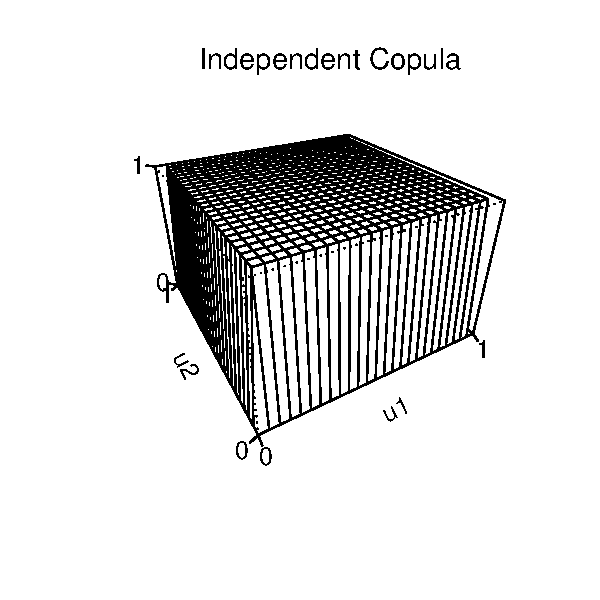
\includegraphics[width=0.4\linewidth]{plots/numerical_results/frank0}
					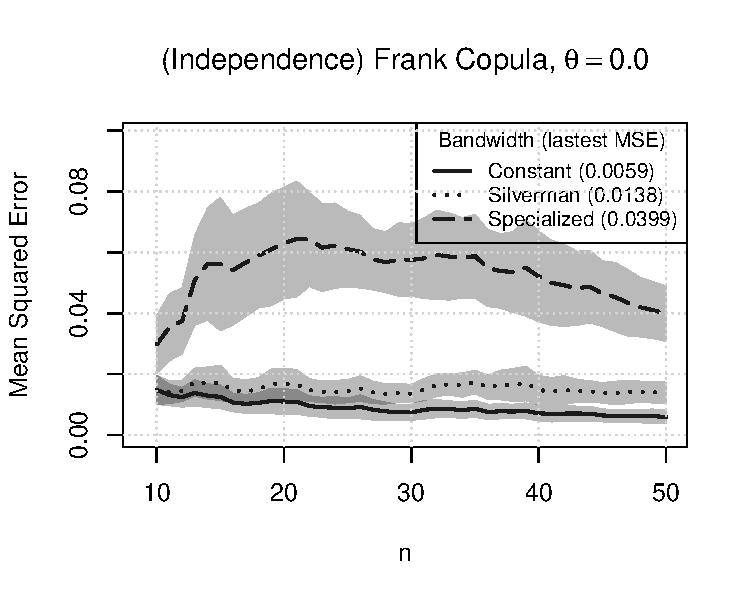
\includegraphics[width=0.5\linewidth]{../text/plots/experiment_results/frank0}
				\end{flushleft}

			\end{frame}
			
		\subsubsection{Student Copula ($ \theta = 0.5 $)}
			\begin{frame}
				\frametitle{\insertsubsubsection}
				
				\begin{flushleft}
					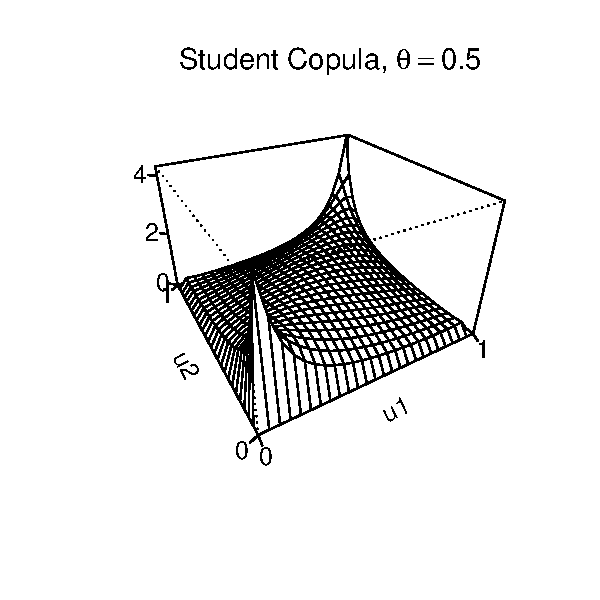
\includegraphics[width=0.4\linewidth]{plots/numerical_results/student05}
					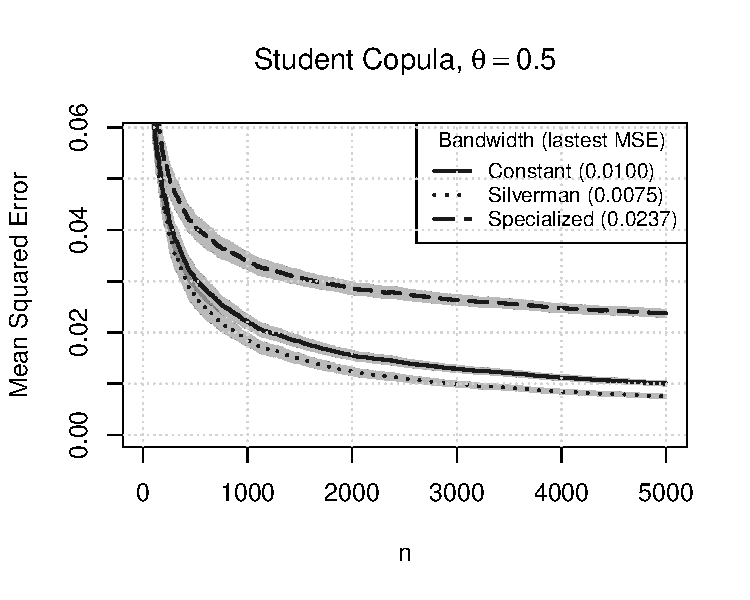
\includegraphics[width=0.5\linewidth]{../text/plots/experiment_results/student05}
				\end{flushleft}
				
			\end{frame}		
			
		
		\subsubsection{Student Copula ($ \theta = 0.0 $)}
			\begin{frame}
				\frametitle{\insertsubsubsection}
				
				\begin{flushleft}
					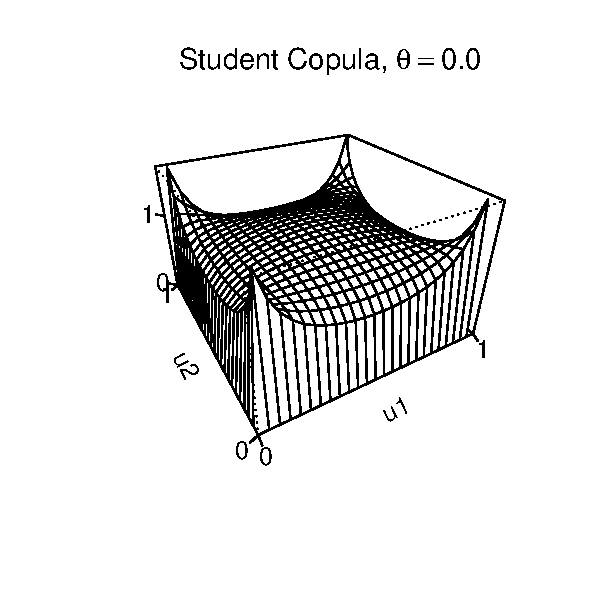
\includegraphics[width=0.4\linewidth]{plots/numerical_results/student0}
					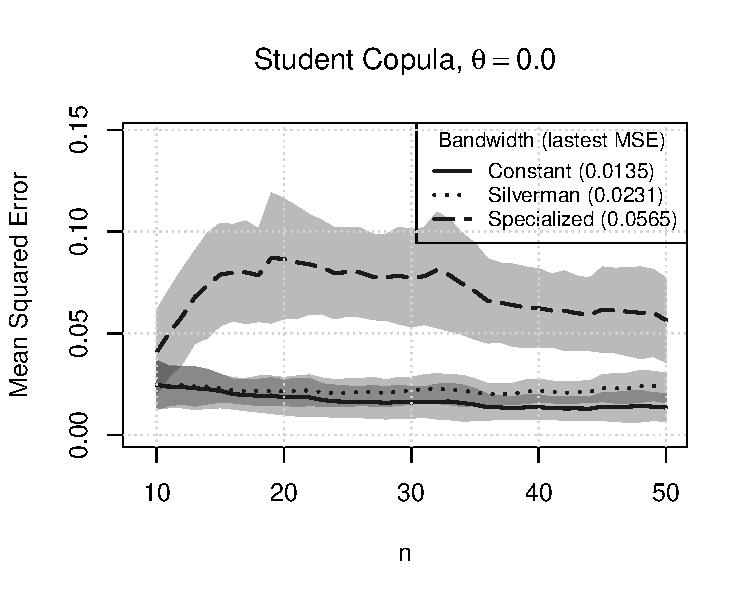
\includegraphics[width=0.5\linewidth]{../text/plots/experiment_results/student0}
				\end{flushleft}
				
			\end{frame}
			
			
		\subsubsection{Clayton Copula ($ \theta = -0.5 $)}
			\begin{frame}
				\frametitle{\insertsubsubsection}
				
				\begin{flushleft}
					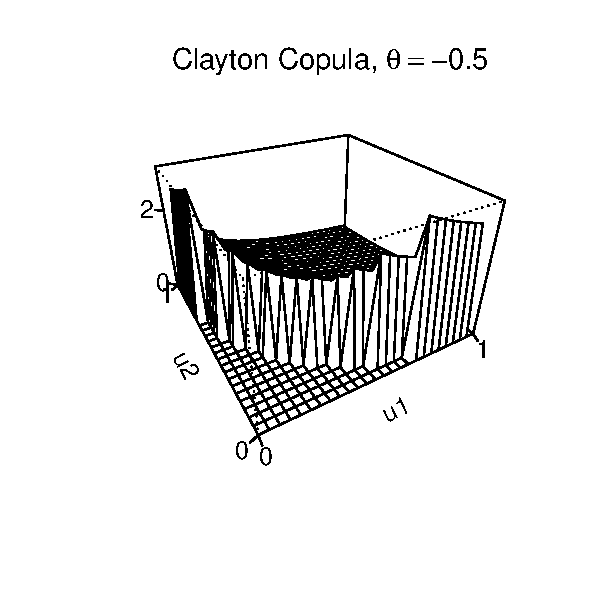
\includegraphics[width=0.4\linewidth]{plots/numerical_results/clayton_05}
					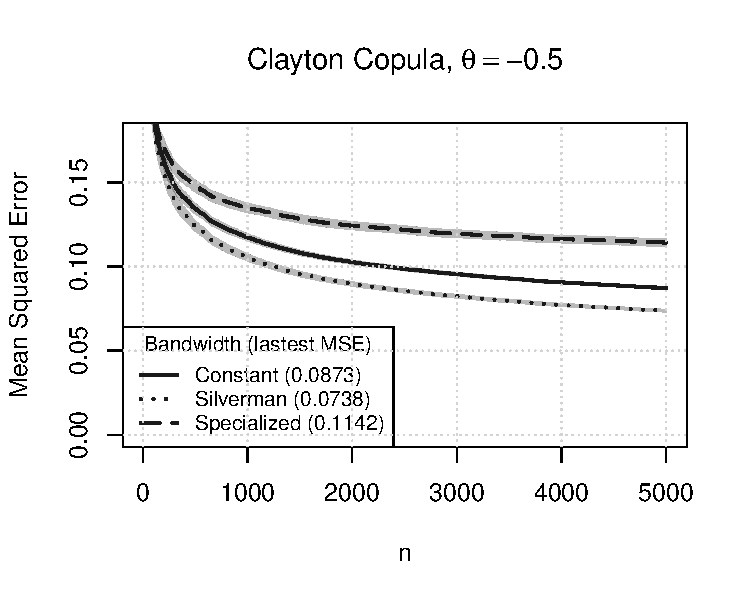
\includegraphics[width=0.5\linewidth]{../text/plots/experiment_results/clayton_05}
				\end{flushleft}
				
			\end{frame}
			
		
		\subsubsection{Clayton Copula ($ \theta = 10 $)}
			\begin{frame}
				\frametitle{\insertsubsubsection}
				
				\begin{flushleft}
					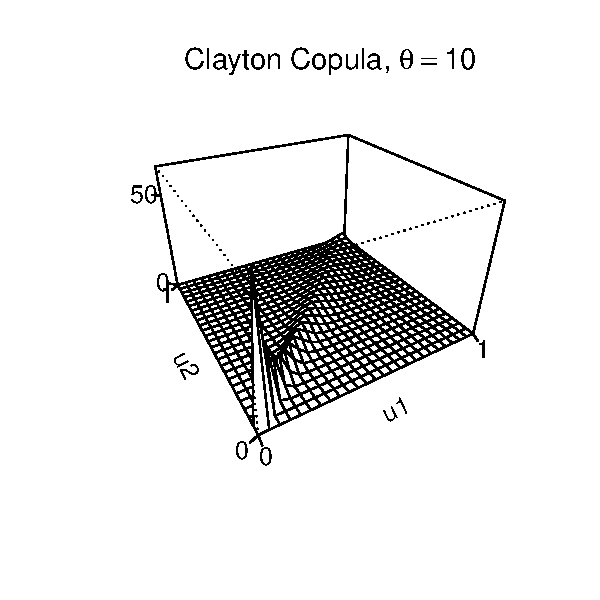
\includegraphics[width=0.4\linewidth]{plots/numerical_results/clayton10}
					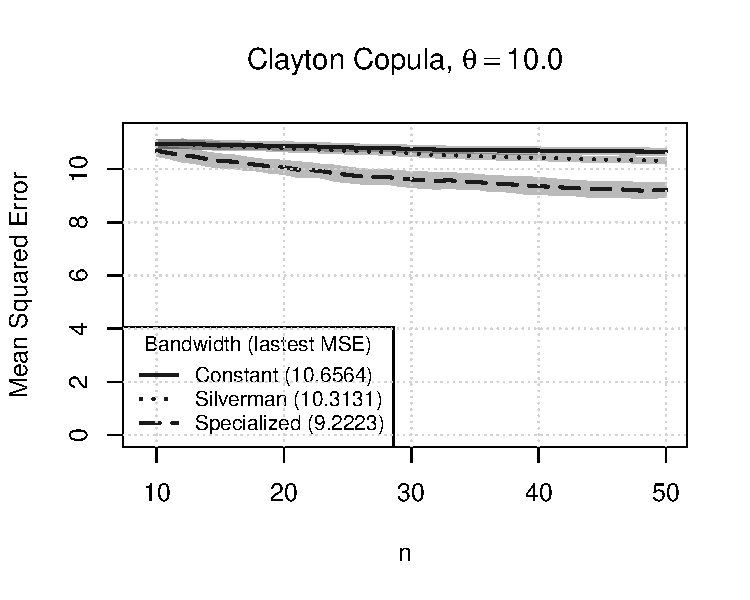
\includegraphics[width=0.5\linewidth]{../text/plots/experiment_results/clayton10}
				\end{flushleft}
				
			\end{frame}
	
		\subsubsection{Numerical results}
			\begin{frame}
				\frametitle{\insertsubsubsection}
				
				\begin{enumerate}
					\item The proposed recursive non-parametric estimator works of copula density works;
					\item<2-> The usage of the constant bandwidths is a good choice;
					\item<3-> Though, data-dependent bandwidths are more reliable in complicated cases.
				\end{enumerate}
				
			\end{frame}
	
\section{Conclusion}
	\begin{frame}
		\frametitle{\insertsection}
		
		Our contribution consists of the following
		\begin{enumerate}
			\item<1-> We introduced the kernel recursive non-parametric estimators of the joint PDF $ f^\mathbf{u} $;
			\item<2-> In addition, using this result we presented the recursive non-parametric estimator of the copula density $ c(\cdot) $;
			\item<3-> Github repository: \href{https://github.com/vdyashin/CopulaDensityEstimator}{\texttt{https://github.com/vdyashin/CopulaDensityEstimator}}.
		\end{enumerate}
		
	\end{frame}
	
\section{Acknowledgements}
	\begin{frame}
		\frametitle{The author sincerely acknowledges}
		
		The university Higher School of Economics for provided opportunity to be an exchange student this semester to meet his professor. \\[1em]
		
		The university staff inc. office managers Maria Neklyudova as well as Ekaterina Pavlova and Ilona Yakovleva for their support and responsiveness. \\[1em]
		
		Special gratitude goes to Felix Camirand (Ph.\,D.) from University of Melbourne who has provided an early version of his paper.\\[1em]
		
		The uncountable number of contributors of \href{https://R-project.org/}{\textbf{R}} package and the creators of the \href{https://cran.r-project.org/web/packages/copula/copula.pdf}{\texttt{copula}} library. The contributors of the \LaTeX~typesetting system are also gratefully acknowledged. 
		
	\end{frame}
			
\section{}
	\maketitle
	~\\[-1em]
	\printbibliography
	
\end{document}